% -*- coding: utf-8 -*-

\chapter{绪论} \label{chpt:introduction}

人工智能的研究历史可追溯至二十世纪中叶，该领域经历了多次高潮与低谷。在2006年，Hinton等人提出的深度学习方法\cite{hinton2006deep}引发了新一轮研究热潮。深度学习之所以能够推动人工智能技术实现质的飞跃，关键在于其在视觉感知、语言理解等复杂任务上展现出的卓越能力，部分场景下甚至超越了人类表现\cite{lecun2015deeplearning}。然而，这一看似强大的技术体系却存在一个致命弱点：对对抗性样本的高度敏感。对抗性样本通过在原始数据上叠加精心设计的细微扰动，可使深度神经网络产生置信度极高但完全错误的判断\cite{szegedy2014intriguing}。Szegedy等人于2014年的实证研究表明，包括当时最先进深度神经网络在内的多种机器学习模型均难以抵御此类攻击\cite{szegedy2014intriguing}。

\section{研究背景和意义}

近年来，深度学习技术在计算机视觉领域取得了举世瞩目的突破性进展\cite{lecun2015deeplearning}。以卷积神经网络为代表的深度模型在图像分类、目标检测、语义分割等核心任务上的表现已全面超越传统方法，甚至在部分基准测试中达到乃至超越人类水平\cite{krizhevsky2012imagenet,he2016resnet}。深度学习模型深刻改变着各行各业的技术格局。

然而，2014年Szegedy等人的开创性研究首次揭示了深度神经网络中普遍存在的对抗样本现象\cite{szegedy2014intriguing}：通过在原始输入图像上叠加人眼几乎无法察觉的微小扰动，便可以使分类能力极强的深度模型以极高置信度输出完全错误的预测结果。如图\ref{fig:adversarial_example}所示，原始图像经过细微扰动处理后得到对抗样本。对于人眼观察者而言，两幅图像视觉上完全一致，均呈现"熊猫"的形象。然而深度神经网络的判断却截然不同：模型对原始输入能够正确分类，却对对抗样本给出了99.3\%置信度的"长臂猿"这一错误预测。

\begin{figure}[htbp]
    \centering
    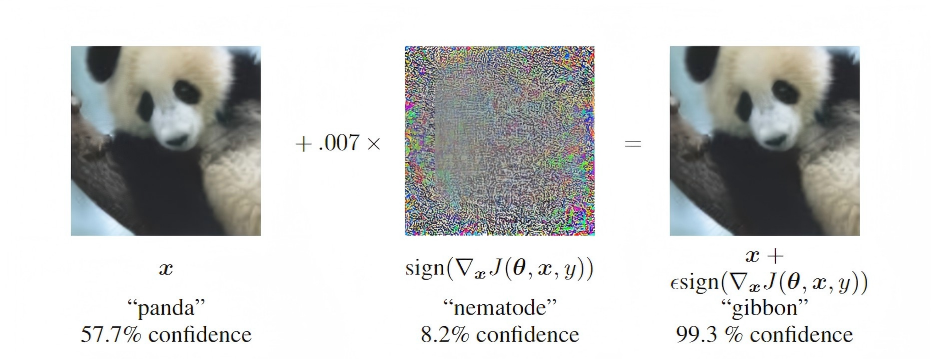
\includegraphics[width=0.8\textwidth]{figures/xiongmao.png}
    \caption{对抗性攻击样本示例}
    \label{fig:adversarial_example}
\end{figure}

这一发现动摇了深度学习系统可靠性高的固有印象，凸显了其固有的脆弱性。后续研究进一步表明，对抗样本的威胁已从数字仿真环境扩展至现实物理世界：Eykholt等人验证了在交通标志上施加特定扰动可诱导自动驾驶系统做出错误决策\cite{eykholt2018robust}，Kurakin 等人进一步证明打印出的对抗样本经手机拍摄后仍能欺骗模型\cite{kurakin2017adversarial}，而医学影像诊断系统中的微弱扰动则可能导致严重误诊\cite{SamuelG.Finlayson2019Adversarial}。这些安全问题表明，开展深度模型对抗鲁棒性研究对于实现人工智能技术的可信部署具有重要意义。

面对对抗样本的挑战，学术界提出了多种防御思路，其中对抗性训练\cite{madry2018pgd}被广泛认为是目前最有效的防御范式。该方法使用对抗性样本进行训练，使得模型增强对扰动的鲁棒性。


\section{国内外研究现状}

\subsection{对抗样本攻击研究现状}

对抗样本攻击方法的研究伴随着深度学习的发展持续演进，形成了从简单到复杂、从数字域到物理域的多元化攻击体系。

在基于梯度的白盒攻击方面，Goodfellow等人提出的快速梯度符号法（FGSM）\cite{goodfellow2015fgsm}是最早的高效攻击算法之一，通过沿损失函数梯度方向施加一步扰动实现攻击，计算代价低但攻击成功率有限。Madry等人将攻击问题形式化为约束优化问题，提出的投影梯度下降攻击（PGD）\cite{madry2018pgd}通过多步迭代逼近最优对抗扰动，被公认为Lp范数约束下最强的一阶攻击方法，至今仍是对抗鲁棒性研究的基准参照。Croce与Hein提出的AutoAttack\cite{croce2020autoattack}将多种互补攻击策略集成为标准化评估框架，有效规避了单一攻击方法评估的局限性，已成为对抗鲁棒性基准评测的通行标准。

在更贴近物理世界的攻击方面，Brown等人提出的对抗补丁攻击（Adversarial Patch）\cite{brown2017adversarialpatch}通过在图像的局部矩形区域叠加显著可见的对抗图案实现攻击，对遮蔽类攻击场景具有直接的启示意义。Eykholt等人进一步证明，在交通标志上物理粘贴特定图案可稳定欺骗自动驾驶视觉系统\cite{eykholt2018robust}，将对抗攻击的威胁从数字仿真推向真实部署场景。在黑盒攻击方面，Tram\`{e}r等人揭示了对抗样本的跨模型可迁移性\cite{tramer2018ensemble}，表明在代理模型上生成的对抗扰动可有效迁移至未知目标模型，从而实现无需访问目标模型梯度的黑盒攻击，大幅降低了现实攻击的实施门槛。

\subsection{对抗性防御研究现状}

对抗性防御方法的研究与攻击方法的进化相互促进，形成了攻防博弈的持续演进格局。

对抗性训练是目前被广泛认可的最有效防御方法。Madry等人提出的标准对抗性训练（PGD-AT）\cite{madry2018pgd}在每轮训练迭代中以PGD生成的对抗样本替换干净样本进行训练，显著提升了模型对梯度攻击的鲁棒性，奠定了对抗性训练的基础范式。然而，PGD-AT的计算开销巨大，制约了其在大规模任务上的应用。Shafahi等人提出的Free-AT\cite{shafahi2019free}通过"免费"复用梯度信息同步更新模型参数与对抗扰动，将训练代价降低至与标准训练相近的水平。Wong等人提出的Fast-AT\cite{wong2020fast}采用随机初始化的FGSM攻击替代多步PGD，在损失较小的精度代价下大幅缩短了训练时间。

在其他防御路径方面，Papernot等人提出的防御蒸馏方法\cite{papernot2016distillation}通过知识蒸馏平滑模型的输出分布，降低对梯度信息的敏感性以缓解梯度攻击的威胁。Cohen等人提出的随机平滑认证防御（Certified Defense）\cite{cohen2019certified}通过对输入施加高斯噪声并统计预测分布，为模型鲁棒性提供可证明的理论保证，是目前为数不多具有严格理论背书的防御方法。M\"{u}ller等人研究了标签平滑正则化在对抗鲁棒性提升中的作用\cite{muller2019labelsmoothing}，证明了正则化手段对模型泛化鲁棒性的积极影响。

然而，综观现有防御研究，绝大多数工作的训练信号仍局限于Lp范数约束下的梯度攻击，对以遮蔽为代表的语义驱动型攻击的防御研究严重不足。这一现状导致经过标准对抗性训练的模型在面对遮蔽攻击时防御能力大幅下降，亟需专门的防御方法加以应对。

\subsection{显著性图与特征归因方法研究现状}

特征归因（Feature Attribution）方法旨在解释深度神经网络的决策过程，通过识别对预测结果具有关键影响的输入特征区域，为模型可解释性研究提供重要工具，同时也为基于语义特征的对抗攻击提供了方法论支撑。

原始梯度显著性图（Vanilla Gradient Saliency）由Simonyan等人率先提出\cite{simonyan2014saliency}，其核心思想是将网络输出对输入的梯度绝对值作为各像素重要性的度量。该方法计算简洁，仅需一次反向传播即可获得全图的重要性评分，是计算效率最高的特征归因方法之一。Sundararajan等人提出的梯度积分（Integrated Gradients, 积分梯度归因）\cite{sundararajan2017ig}在梯度显著性图的基础上引入了公理化约束，通过沿基线到输入的路径对梯度进行积分，满足灵敏性与实现不变性等理论性质，归因精度显著优于原始梯度方法，但代价是需要多次前向与反向传播，计算开销远高于原始梯度显著性图。Selvaraju等人提出的梯度加权类激活映射（Grad-CAM）\cite{selvaraju2017gradcam}利用卷积特征图的梯度生成类别区分性热力图，能够在不改变网络结构的前提下直观呈现模型的视觉关注区域，在网络可解释性可视化领域得到了广泛应用。

上述特征归因方法具有重要的攻击应用潜力：通过识别模型判断的关键像素区域，可以有针对性地在这些高显著性位置施加遮蔽扰动，从而以最小的扰动面积实现最大化的攻击效果。本文同时实现了基于原始梯度显著性图与梯度积分（积分梯度归因）两种归因方法的遮蔽攻击，系统对比了两种方法在攻击效果、计算效率及对抗训练中的差异。实验表明，积分梯度归因归因的遮蔽攻击在归因精度上更优，攻击强度更高，但计算代价约为梯度显著性图的数十倍。


\section{研究的关键问题}

遮蔽攻击作为对抗攻击的一种重要形式，目前相关研究相对匮乏。本文将着重于基于特征归因图的遮蔽攻击及其对抗性训练方法的研究，从以下三个方面具体展开：遮蔽攻击的设计与实现，对抗性训练策略的构建，防御性能的评估与影响因素分析。

\subsection{遮蔽攻击的设计与实现}

遮蔽攻击的核心在于识别图像中对模型判断起关键作用的区域，并在该区域施加遮蔽扰动。本文实现了两种归因方法来生成显著性图：基于梯度积分（积分梯度归因）的方法和基于梯度显著性图的方法。在此基础上，本文设计了固定遮蔽攻击和自适应遮蔽攻击两种攻击变体，并对两种方法的攻击效果进行对比分析，为后续防御研究提供攻击样本来源。

\subsection{对抗性训练策略的构建}

对抗性训练被广泛认为是最有效的防御方法。然而，现有对抗性训练方法主要针对$L_p$范数约束下的梯度攻击设计，对遮蔽攻击的防御能力不足。本文需要设计一种针对遮蔽攻击的对抗性训练策略，同时兼顾模型对干净样本的识别准确率。此外，本文还提出了混合对抗性训练策略，将遮蔽攻击与PGD攻击相结合，以提升模型在多类型攻击场景下的泛化防御能力。

\subsection{防御性能的评估与影响因素分析}

对抗性训练策略实现后，对其防御性能的评估与分析同样重要。本文需要建立合理的评估指标，对所提出的防御策略进行系统测试。在此基础上，还需要分析攻击参数（如遮蔽区域大小、遮蔽块数量）对防御性能的影响，以及不同训练策略之间的效果差异，从而为遮蔽攻击防御领域的后续研究提供参考。


\section{论文的主要工作}

针对1.3节中提出的问题，本文使用不同归因方法设计了遮蔽攻击方法，并提出了相应的对抗性训练策略。在MNIST数据集上对所提方法进行了实验验证，分析了不同参数设置对攻防性能的影响。本文的主要工作如下：

1) 介绍了显著性图与特征归因方法的基本原理，同时实现了基于梯度显著性图和梯度积分（积分梯度归因）两种归因方法的遮蔽攻击。在此基础上，分别设计了固定遮蔽攻击和自适应遮蔽攻击两种攻击变体，系统对比了两种归因方法在攻击效果与计算效率上的差异。

2) 基于LeNet-5神经网络模型，实现了所提出的遮蔽攻击算法。通过特征归因图定位图像中对模型判断起关键作用的像素区域，在这些区域施加遮蔽块，从而干扰模型的分类判断。

3) 设计了针对遮蔽攻击的对抗性训练策略，并提出将遮蔽攻击与梯度攻击相结合的混合对抗性训练方案（Mix-AT）。在每轮训练迭代中同时引入两类对抗样本，使模型在保持对梯度类攻击鲁棒性的同时，提升对遮蔽类攻击的防御能力。

4) 对所提方法进行了系统的实验评估。在MNIST数据集上对九种防御策略（涵盖显著性归因与积分梯度归因两类遮蔽训练）在七类攻击下进行了对比测试，分析了遮蔽参数对攻击效果的影响。实验验证了原始梯度显著性遮蔽攻击与梯度攻击在混合训练模型上呈现抵消效应\cite{Duan2023InequalityPI}。


\section{论文组织结构}

本文共分为五章，各章节内容如下：

\textbf{第一章：绪论}。介绍深度学习安全性研究的背景与意义，系统梳理对抗样本攻击、对抗性防御以及显著性图与特征归因方法的国内外研究现状，指出研究的关键问题并概述本文的主要工作，最后给出论文组织结构。

\textbf{第二章：相关理论与技术基础}。介绍本文所涉及的核心技术原理，包括深度神经网络的基本结构与训练原理、对抗样本的定义与威胁模型、常见对抗攻击方法的数学表述，以及显著性图与特征归因方法的理论基础，为后续章节的方法设计提供理论支撑。

\textbf{第三章：基于特征归因图的遮蔽攻击与对抗性训练方法}。详细阐述本文提出的方法体系，包括基于梯度显著性图的固定遮蔽攻击算法设计、自适应遮蔽攻击的逐样本早停机制，以及将遮蔽攻击与PGD攻击相结合的混合对抗性训练策略的完整实现方案。

\textbf{第四章：实验与结果分析}。介绍实验环境配置、数据集选取与评估指标设定，对多种防御策略在攻击类型下的鲁棒性进行系统对比分析，并开展攻击参数敏感性分析与迁移攻击鲁棒性验证实验，深入讨论所提方法的有效性及局限性。

\textbf{第五章：总结与展望}。总结本文的主要工作与核心结论，分析现有研究的局限性，并对未来可能的研究方向进行展望。
